\documentclass[11pt, a4paper]{article}
\usepackage[a4paper, margin=1in]{geometry}

\usepackage{adjustbox}
\usepackage{mathtools}
\usepackage{amsmath}
\usepackage{amssymb}
\usepackage{amsthm}
\usepackage{tkz-euclide}

\usepackage{pgfplots}
\usepackage{listings}
\usepackage{color}
\usepackage{tikz}

\usepackage{textcomp}
\usepackage{soul}

\usepackage[hidelinks]{hyperref}
\pgfplotsset{width=7.5cm,compat=1.12}
\usepgfplotslibrary{fillbetween}
\pgfplotsset{compat=1.8}
\usepgfplotslibrary{statistics}
\usepackage[makeroom]{cancel}
\title{\bf{Homework \textnumero 9}}
\author{Author: David Oniani
\\
\ \ \ Instructor: Dr. Eric Westlund}
\date{March 9, 2019}

\usepackage{listings}
\usepackage{color}

%%%%%%%%%%%%%%% S E T S %%%%%%%%%%%%%%%
\newcommand{\nats}{\mathbb{N}}
\newcommand{\ints}{\mathbb{Z}}
\newcommand{\rats}{\mathbb{Q}}
\newcommand{\reals}{\mathbb{R}}
\newcommand{\irrats}{\mathbb{I}}

\newcommand{\pnats}{\mathbb{N}^+}
\newcommand{\pints}{\mathbb{Z}^+}
\newcommand{\prats}{\mathbb{Q}^+}
\newcommand{\preals}{\mathbb{R}^+}
\newcommand{\nreals}{\mathbb{R}^-}

\newcommand{\nints}{\mathbb{Z}^-}
\newcommand{\nrats}{\mathbb{Q}^-}
%%%%%%%%%%%%%%%%%%%%%%%%%%%%%%%%%%%%%%%

% Calligraphy
\newcommand\und[1]{\underline{\smash{#1}}}

% Operators
\DeclarePairedDelimiter\abs{\lvert}{\rvert}
\DeclarePairedDelimiter\ceil{\lceil}{\rceil}
\DeclarePairedDelimiter\floor{\lfloor}{\rfloor}

% Other
\newcommand{\rarr}{\rightarrow}

\definecolor{dkgreen}{rgb}{0,0.6,0}
\definecolor{gray}{rgb}{0.5,0.5,0.5}
\definecolor{mauve}{rgb}{0.58,0,0.82}
\definecolor{backcolour}{rgb}{0.95,0.95,0.92}

\lstset{
backgroundcolor=\color{backcolour},
aboveskip=3mm,
belowskip=3mm,
showstringspaces=false,
columns=flexible,
basicstyle={\small\ttfamily},
numbers=left,
numberstyle=\normalsize\color{gray},
keywordstyle=\color{blue},
commentstyle=\color{dkgreen},
stringstyle=\color{mauve},
breaklines=true,
breakatwhitespace=true,
tabsize=4
}


\begin{document}
\maketitle
\begin{itemize}
\item[12.10]
\begin{itemize}
\item[(a)]
It is $0.083 + 0.789 = 0.872$.

\item[]

\item[(b)]
It should be $1 - 0.083 - 0.789 = 0.128$.

\item[]

\item[(c)]
It is $1 - 0.083 = 0.917$.
\end{itemize}

\item[]
\item[]

\item[12.12]
Notice that in models 1, 3, and 4, the probabilities do not add up to 1.\\\\
In model 1, we have $\dfrac{1}{7} + \dfrac{1}{7} + \dfrac{1}{7} + \dfrac{1}{7} + \dfrac{1}{7} + \dfrac{1}{7} = \dfrac{6}{7} < 1$.\\\\
In model 3, we have $\dfrac{1}{3} + \dfrac{1}{6} + \dfrac{1}{6} + \dfrac{1}{6} + \dfrac{1}{6} + \dfrac{1}{6} = \dfrac{7}{6} > 1$.\\\\
In model 4, we have $1 + 1 + 2 + 1 + 1 + 2 = 8 > 1$.\\\\
Model 2 seems perfectly reasonable as $\dfrac{1}{3} + \dfrac{1}{6} + \dfrac{1}{6} + 0 + \dfrac{1}{6} + \dfrac{1}{6} = 1$.\\\\
Finally, we conclude that models 1, 3, and 4 are invalid while model 2 is valid.

\item[]
\item[]

\item[12.13]
\begin{itemize}
\item[(a)]
$A = \{4, 5, 6, 7, 8, 9\}, \ \text{P}(A) = 6/10 = 0.6$.
\item[]

\item[(b)]
$B = \{0, 2, 4, 6, 8\}, \ \text{P}(B) = 5/10 = 0.5$ (this assumes that $05 = 5$; otherwise $B = \{2, 4, 6, 8\}$and $\text{P}(B) = 4/10 = 0.4$).

\item[]

\item[(c)]
$\text{$A$ or $B$} = \{4, 5, 6, 7, 8, 9\} \cup \{0, 2, 4, 6, 8\} = \{0, 2, 4, 5, 6, 7, 8, 9\}$.\\
\vspace{0.005cm}\\
$\text{P$(A$ or $B)$} = \text{P}(A) + \text{P}(A) - \text{P}(A \cap B) = \dfrac{8}{10} = 0.8$.\\
\vspace{0.005cm}\\
The probability is not equal to $\text{P}(A) + \text{P}(B)$ as $A$ and $B$ are not disjoint.
\end{itemize}

\newpage

\item[12.15]
\begin{itemize}
\item[(a)]
$\text{P}(Y \leq 0.6) = \text{P}(0 \leq Y \leq 0.6) = 0.6 - 0 = 0.6$.

\item[]

\item[(b)]
$\text{P}(Y < 0.6) = \text{P}(0 \leq Y < 0.6) = 0.6 - 0 = 0.6$.

\item[]

\item[(c)]
$\text{P}(0.4 \leq Y \leq 0.8) = 0.8 - 0.4 = 0.4$.

\item[]

\item[(d)]
$\text{P}(0.4 < Y \leq 0.8) = 0.8 - 0.4 = 0.4$.
\end{itemize}

\item[]
\item[]

\item[12.16]
\begin{itemize}
\item[(a)]
$S = \dfrac{ah}{2} = \dfrac{(2 - 0) \times 1}{2} = \dfrac{2}{2} = 1$.

\item[]

\item[(b)]
The probability is the half of the area of the triangle and therefore is $\dfrac{1}{2} = 0.5$.

\begin{figure}[h]
    \centering
    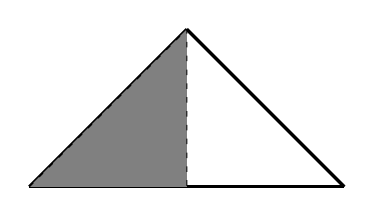
\begin{tikzpicture}[scale=0.5]
        \draw [very thick] (0, 0) -- (8, 0);
        \draw [very thick] (0, 0) -- (4, 4);
        \draw [very thick] (8, 0) -- (4, 4);
        \draw [fill=gray, dash pattern=on 2pt off 3pt] (0, 0) -- (4, 4) -- (4, 0);
    \end{tikzpicture}
\end{figure}

\item[]

\item[(c)]
The probability is the eighth of the area of the triangle and therefore is $\dfrac{1}{8} = 0.125$.

\begin{figure}[h]
    \centering
    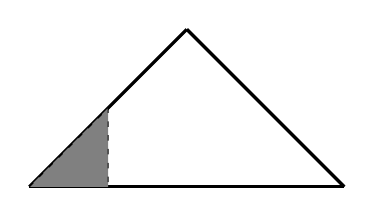
\begin{tikzpicture}[scale=0.5]
        \draw [very thick] (0, 0) -- (8, 0);
        \draw [very thick] (0, 0) -- (4, 4);
        \draw [very thick] (8, 0) -- (4, 4);
        \draw [fill=gray, dash pattern=on 2pt off 3pt] (0, 0) -- (2, 2) -- (2, 0);
    \end{tikzpicture}
\end{figure}
\end{itemize}

\item[]
\item[]

\item[12.17]
\begin{itemize}
\item[(a)]
$\chi \geq 35$.

\item[]

\item[(b)]
Let's first find the $z$-score. We get $z = \dfrac{x - \mu}{\sigma} = \dfrac{35 - 25.3}{6.5} \approx 1.49$.\\
From the table A, we get that the corresponding area to the left is $0.9319$. Finally, we
get that the probability is $1 - 0.9319 = 0.0681 \approx 0.07$.
\end{itemize}

\item[]
\item[]

\item[12.20]
\begin{itemize}
\item[(a)]
Since currently I am not an active driver and spend most of my time on campus, I expect it to be less than 0.2.
I predict it to be 0.05.

\item[]

\item[(b)]
As I stated in the part (a) of the exercise, I virtually do not drive and spend most of the time on campus.
This is the primary reason why the chance is lower than the ``average'' probability of 0.2.

\item[]

\item[(c)]
That's the nature of a human. People hope that they won't be in an accident and are feared by a mere thought
of being in it. Because of this, most people say that the chance of the accident is really low (below 0.2).
\end{itemize}

\item[]
\item[]

\item[12.32]
\begin{itemize}
\item[(c)]
$S$ = \{MMMM, HMMM, MHMM, MMHM, MMMH, HMMH, HHMM, MHHM,\\
MMHH, MHMH, HMHM, MHHH, HMHH, HHMH, HHHM, HHHH\}.

\item[]

\item[(b)]
$S = \{0, 1, 2, 3, 4\}$
\end{itemize}

\item[]
\item[]

\item[12.34]
\begin{itemize}
\item[(a)]
The probability would be $\text{P$($some education beyond high school but no bachelor's degree$)$} = 1 - 0.1 - 0.27 - 0.34 = 0.29$.

\item[]

\item[(b)]
The probability would be $1 - 0.1 = 0.9$.
\end{itemize}

\item[]
\item[]

\item[12.37]
\begin{itemize}
\item[(a)]
It would be $1 - 0.25 - 0.18 - 0.18 - 0.12 - 0.09 - 0.08 - 0.07 = 0.03$.
\item[]

\item[(b)]
It would be $1 - 0.25 - 0.18 = 0.57$.
\end{itemize}

\item[]
\item[]

\item[12.47]
\begin{itemize}
\item[(a)]
$S$ = \{$($Abby, Deborah$)$, $($Abby, Mei-Ling$)$, $($Abby, Sam$)$, $($Abby, Roberto$)$,\\
$($Deborah, Mei-Ling$)$, $($Deborah, Sam$)$, $($Deborah, Roberto$)$, $($Mei-Ling, Sam$)$,\\
$($Mei-Ling, Roberto$)$, $($Sam, Roberto$)$\}

\item[]

\item[(b)]
Each has the probability of $\dfrac{1}{10} = 0.1$.

\item[]

\item[(c)]
Notice that Mei-Ling is chose in 4 out of 10 outcomes.\\
\vspace{0.00125cm}\\
Therefore $\text{P$($Mei-Ling is chosen$)$} = \dfrac{4}{10} = 0.4$.

\item[]

\item[(d)]
Notice that there are, in total, 3 pairs without Sam and Roberto (namely, $($Abby, Deborah$)$, $($Abby, Mei-Ling$)$, and $($Deborah, Mei-Ling$)$).\\
Therefore, $\text{P$($both people selected liked the course$)$} = \dfrac{3}{10} = 0.3$.
\end{itemize}

\newpage

\item[12.51]
\begin{itemize}
\item[(a)]
The random variable $Y$ is continuous.\\
This is because the set of possible values is the interval which means that the values can be decimals.

\item[]

\item[(b)]
The height has to be $\dfrac{1}{2}$ because the total area must be 1.\\
Below is the density curve.
\begin{figure}[h]
    \centering
    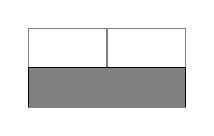
\begin{tikzpicture}
        \tkzInit[xmax=2,ymax=1,xmin=0,ymin=0]
        \tkzGrid
        \tkzAxeXY
        \draw [fill=gray] (0, 0) -- (0, 0.5) -- (2, 0.5) -- (2, 0);

    \end{tikzpicture}
\end{figure}
\end{itemize}

\item[]

\item[(c)]
$\text{P}(Y \leq 1) = \dfrac{2 \times \dfrac{1}{2}}{2} = \dfrac{1}{2} = 0.5$.

\item[]
\item[]

\item[12.52]
\begin{itemize}
\item[(a)]
$\text{P}(0.5 < Y < 1.3) = (1.3 - 0.5) \times 0.5 = 0.8 \times 0.5 = 0.4$.

\item[]

\item[(b)]
$\text{P}(Y \geq 0.8) = (2 - 0.8) \times 0.5 = 1.2 \times 0.5 = 0.6$.
\end{itemize}

\end{itemize}

\end{document}
